\documentclass{standalone}% For the example only, any class will do

  \usepackage{tikz}
  \usetikzlibrary{positioning}% To get more advances positioning options
  \usetikzlibrary{arrows}% To get more arrow heads
  
  \begin{document}

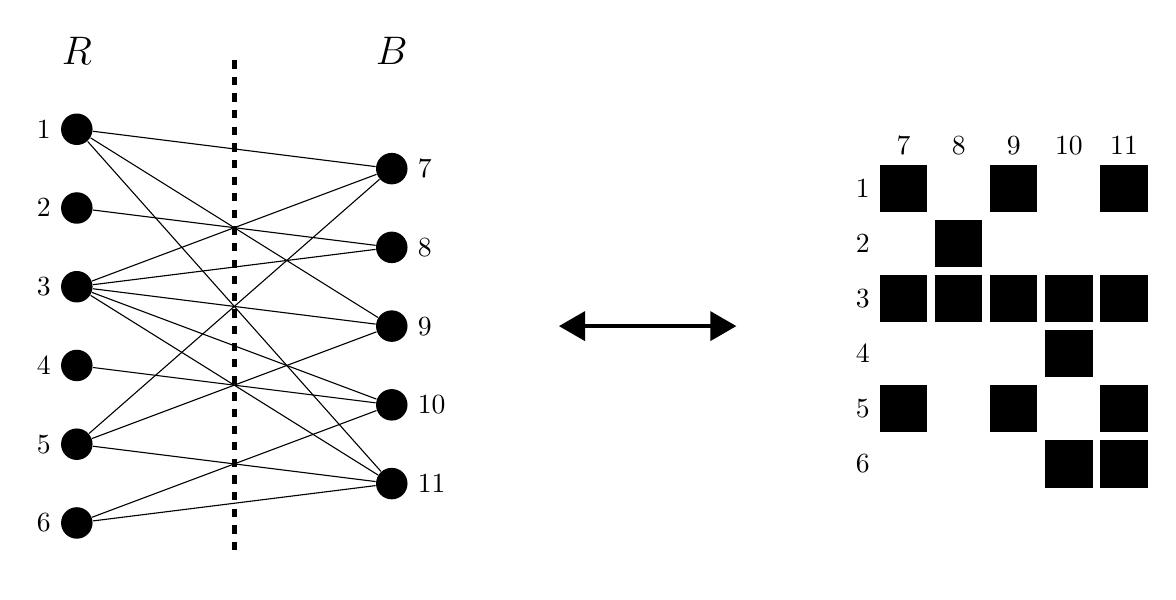
\begin{tikzpicture}

\tikzstyle{thickline} = [ultra thick, dashed]
\tikzstyle{circlenode} = [circle, thin, fill, minimum size=4mm]
\tikzstyle{squarenode} = [thin, fill, minimum size=6mm]
\tikzstyle{myedgestyle} = [ultra thick, -triangle 60]
\def\x{0.7}

\begin{scope}[xshift=-7cm,yshift=0.25cm]
  \node [circlenode] (v1) at (-3.5,4) [label=left:$1$]{};
  \node [circlenode] (v8) at (-3.5,3) [label=left:$2$]{};
  \node [circlenode] (v5) at (-3.5,2) [label=left:$3$]{};
  \node [circlenode] (v9) at (-3.5,1) [label=left:$4$]{};
  \node [circlenode] (v6) at (-3.5,0) [label=left:$5$]{};
  \node [circlenode] (v11) at (-3.5,-1) [label=left:$6$]{};
  \node [circlenode] (v7) at (0.5,3.5) [label=right:$7$]{};
  \node [circlenode] (v4) at (0.5,2.5) [label=right:$8$]{};
  \node [circlenode] (v2) at (0.5,1.5) [label=right:$9$]{};
  \node [circlenode] (v10) at (0.5,0.5) [label=right:$10$]{};
  \node [circlenode] (v3) at (0.5,-0.5) [label=right:$11$]{};
  \draw  (v1) edge (v2);
  \draw  (v1) edge (v7);
  \draw  (v1) edge (v3);
  \draw  (v7) edge (v5);
  \draw  (v4) edge (v5);
  \draw  (v2) edge (v5);
  \draw  (v10) edge (v5);
  \draw  (v3) edge (v5);
  \draw  (v6) edge (v7);
  \draw  (v8) edge (v4);
  \draw  (v9) edge (v10);
  \draw  (v11) edge (v10);
  \draw  (v3) edge (v6);
  \draw  (v3) edge (v11);
  \draw  (v6) edge (v2);
  \node (v12) at (-1.5,5) {};
  \node (v13) at (-1.5,-1.5) {};
  \draw [thickline] (v12) edge (v13);
  \node at (-3.5,5) {\Large$R$};
  \node at (0.5,5) {\Large$B$};
\end{scope}

\begin{scope}[xshift=0cm]
  \node [squarenode] at (0*\x,0*\x) [label=left:$6$,opacity=0]{};
  \node [squarenode] at (0*\x,1*\x) [label=left:$5$]{};
  \node [squarenode] at (0*\x,2*\x) [label=left:$4$,opacity=0]{};
  \node [squarenode] at (0*\x,3*\x) [label=left:$3$]{};
  \node [squarenode] at (0*\x,4*\x) [label=left:$2$,opacity=0]{};
  \node [squarenode] at (0*\x,5*\x) [label=left:$1$,label=above:$7$]{};
  \node [squarenode] at (1*\x,3*\x) {};
  \node [squarenode] at (1*\x,4*\x) {};
  \node [squarenode] at (1*\x,5*\x) [label=above:$8$,opacity=0]{};
  \node [squarenode] at (2*\x,1*\x) {};
  \node [squarenode] at (2*\x,3*\x) {};
  \node [squarenode] at (2*\x,5*\x) [label=above:$9$]{};
  \node [squarenode] at (3*\x,0*\x) {};
  \node [squarenode] at (3*\x,2*\x) {};
  \node [squarenode] at (3*\x,3*\x) {};
  \node [squarenode] at (3*\x,5*\x) [label=above:$10$,opacity=0]{};
  \node [squarenode] at (4*\x,0*\x) {};
  \node [squarenode] at (4*\x,1*\x) {};
  \node [squarenode] at (4*\x,3*\x) {};
  \node [squarenode] at (4*\x,5*\x) [label=above:$11$]{};
  
\end{scope}
  
\begin{scope}[xshift=-3.5cm,yshift=1.75cm]
  \node (v1) at (0,0) {};
  \node (v2) at (1.5,0) {};
  \draw [myedgestyle] (v1) edge (v2);
  \node (v8) at (-1,0) {};
  \node (v9) at (0.5,0) {};
  \draw [myedgestyle] (v9) edge (v8);
\end{scope}

\end{tikzpicture}
\end{document}